\subsection{Background}
The Discrete Fourier Transform (DFT) is a mathematical tool used in signal processing and many other fields. It transforms a sequence of complex numbers, which represent samples of a signal in its time domain, into another sequence of complex numbers. The resulting sequence is said to be its frequency domain representation and it has multiple interesting properties.

The Fast Fourier Transform (FFT)\cite{fft_algorithms_1}\cite{fft_algorithms_2} is crucial for its efficiency in analyzing signals by quickly breaking them down into their frequency components. This computational speed makes FFT essential in real-time applications, such as telecommunications and audio processing, where rapid signal analysis is paramount. In fact, it is not an overstatement to say that the FFT changed the world, revolutionizing many industries. It plays a vital role in spectral analysis\cite{fft_application_3}\cite{fft_application_4}, image processing\cite{fft_application_5}, communication systems\cite{fft_application_1}, biomedical applications\cite{fft_application_6}, audio processing\cite{fft_application_2}, and data compression\cite{fft_application_7}. The FFT's ability to efficiently reveal and manipulate frequency information has wide-ranging implications across various fields, making it a fundamental tool in signal processing and analysis.

\subsection{Code structure and functionalities}
The code for all 1D and 2D CPU Fourier Transform implementations can be found in the files \texttt{Fourier\-Transform.cpp}, \texttt{Fourier\-Transform\-Calculator.cpp} and \texttt{Bit\-Reversal\-Permutation.cpp}, which form the core of our codebase. 

All of our 1D DFT implementations inherit from an abstract class named \texttt{Fourier\-Transform\-Algorithm}, so that a common interface for all 1D DFT algorithms could be given. The class defines a virtual operator, which is overridden by its implementations, defining the main computations for both the direct and the inverse algorithm. The direct and inverse algorithms can then be called using the class \texttt{Fourier\-Transform\-Calculator}, which is passed a unique pointer to a \texttt{Fourier\-Transform\-Algorithm} and has two methods that can be used for performing the direct and inverse DFT respectively. 

The 2D DFT and CUDA implementations will be better explained in Section \ref{sec:cuda}.

\subsubsection{Fourier transform algorithms}
The first DFT implementation we developed can be found in the class \texttt{Classical\-Fourier\-Transform\-Algorithm}, which implements the well-known $O(n^2)$ DFT.  A second implementation is located in the class \texttt{Recursive\-Fourier\-Transform\-Algorithm} and, as the names suggests, it calculates the fast Fourier transform of a sequence using recursion and has time complexity $O(n log(n))$. 

After analyzing the recursion tree, it can be understood that, if we reorder the elements of the sequence in a way that corresponds to the indexes obtained in the leaves of the recursion tree, we can do the computations in an iterative way instead of recursively. The reordering of the elements is done in the \texttt{Bit\-Reversal\-Permutation\-Algorithm} class and will be explained in the next section. After reordering the elements, the rest of the computations can be done by a simple for loop that goes through all the levels of the recursion tree, computes even and odd coefficients of the final answer in each level and then combines them into a single result. The class \texttt{Iterative\-Fourier\-Transform\-Algorithm} implements said algorithm and has the same asymptotical complexity, but performs a lot better in practice and is more easily parallelizable.

In fact, after further analysis, we realized that the computations in each layer of the recursion tree can be done in parallel, as there is no computational dependency between them. The tool we used was OpenMP. By using \texttt{\#pragma omp parallel for}, the calculations could be split among each core or hardware thread of the processor. We then further optimized the memory access by identifying variables that could be privatized for each thread and used the \texttt{firstprivate} clause to make them private to each thread. We then swapped divisions for bit shifts, removed unnecessary computations and used multiplications in place of \texttt{std::abs} whenever possible, to further increase the performance gain.

\subsubsection{Bit reversal permutation algorithms}
We implemented three different bit reversal permutation algorithms. The class \texttt{Naive\-Bit\-Reversal\-Permutation\-Algorithm} contains a naive implementation, used for testing for correctness. The class \texttt{Mask\-Bit\-Reversal\-Permutation\-Algorithm} was adapted from \cite{mask_bit_rev} and follows a similar approach, but it is made more efficient using biwise operators, bit masks and bit shifts. Both these implementations have a time complexity of $O(n log(n))$, but the latter has a very small constant. Moreover, both implementations loop over the entire sequence and calculate the bit reversed representation of each index. As such, this loop is easily parallelizable. The third implementation can be found in \texttt{Fast\-Bit\-Reversal\-Permutation\-Algorithm}, it was adapted from \cite{fast_bit_rev} and has a time complexity of $O(n)$. While asymptotically better performing than \texttt{Mask\-Bit\-Reversal\-Permutation\-Algorithm}, this implementation performs worse for small sequences and has worse parallel scaling. 

All implementations were parallelized using OpenMP. Moreover, the implementation in \texttt{Mask\-Bit\-Reversal\-Permutation\-Algorithm} calls the function \texttt{Mask\-Bit\-Reverse} in a loop, which was declared using the pragma \texttt{\#pragma omp declare simd} with some additional clauses, to allow the compiler to more easily perform vectorization.

\subsection{Results}
We performed performance and parallel scaling tests using a consumer-grade device, with an AMD Ryzen 9 5900HX CPU with 8 physical cores, 16GB of DDR4 RAM and using WSL as an operating system. Results for the implementation in \texttt{Iterative\-Fourier\-Transform\-Algorithm} use an instance of \texttt{Mask\-Bit\-Reversal\-Permutation\-Algorithm} for the bit reversal permutation step and are relative to the direct transform. Unless otherwise stated, all sequences used for testing are randomly generated sequences of complex numbers, stored using the \texttt{std::complex<double>} data type.

Using a sequence with $2^{19}$ elements and calculating the minimum execution times over 100 runs, the iterative algorithm with 8 OpenMP threads was $26.55x$ faster than the recursive one and $1.73x$ faster than the one implemented in the library Numpy. While the latter result is likely partially due to the small overhead for using Numpy functions and methods, this shows that our implementation is more than capable of competing with it for sequences of this size. Moreover, with the same number of runs but a sequence of just $2^{12}$ elements, the iterative algorithm is $969.32x$ faster than the $O(n^2)$ implementation. This shows how the introduction of FFT algorithms makes executing the Fourier Transform of a sequence of $2^{19}$ elements computationally simple even on a consumer-grade device, whereas executing the same transform with the $O(n^2)$ implementation would have taken about 18 hours on the same hardware. These results were obtained using the script \texttt{compare-methods.py}.

Moreover, we performed scaling tests with respect to both the number of OpenMP threads and the length of the sequence, using the scripts \texttt{compute\--performance.py} and \texttt{compute\--scaling.py} respectively. In Figure \ref{fig:fft_threads} the average execution time over 1000 runs for a sequence of $2^{19}$ elements can be seen for 1, 2, 4 and 8 OpenMP threads. In Figures \ref{fig:fft_floats} and \ref{fig:fft_doubles} the speed-up trend for multiple sequence lengths for floats and doubles respectively can be seen. Results refer to minimum execution times over 1000 runs.

\begin{figure}[ht]
    \centering
    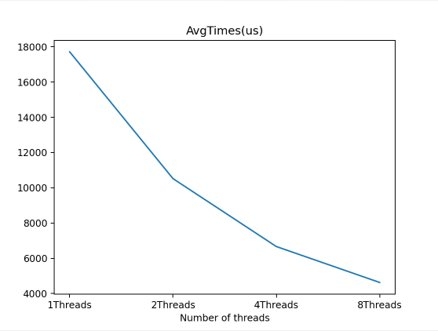
\includegraphics[width=70mm]{image/fft_times}
    \caption{Parallel scaling test with $2^{19}$ elements.}
    \label{fig:fft_threads}
\end{figure}

\begin{figure}[ht]
    \centering
    \subfigure[Speed-ups for floats]{\label{fig:fft_floats}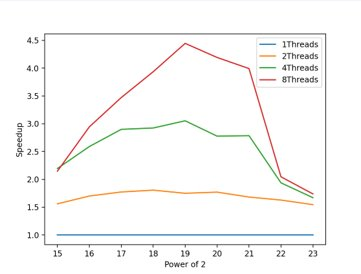
\includegraphics[width=55mm]{image/fft_scaling_floats}}
    \subfigure[Speed-ups for doubles]{\label{fig:fft_doubles}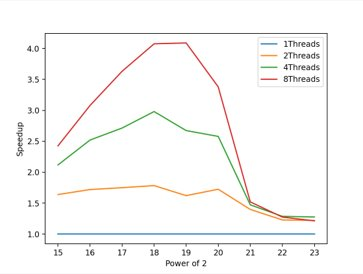
\includegraphics[width=55mm]{image/fft_scaling_doubles}}
    \caption{Scaling test with respect to the sequence length.}
    \label{fig:fft_performance}
\end{figure}

Figures \ref{fig:fft_floats} and \ref{fig:fft_doubles} show the expected trend of increasing speed-up up to a certain number of threads, as the overhead for OpenMP communication is hidden by the larger sequence sizes. However, when reaching $2^{22}$ and $2^{21}$ elements for floats and doubles respectively, the speed-up decreases drastically. We believe this behaviour is related to the size of the L3 cache of the machine, as $2^{21}$ double complex values and $2^{22}$ float complex values both require 32 MB of memory, while the L3 cache of the machine is 16 MB large. We believe that the processor is unable to perform caching effectively due to the complex access pattern to memory, causing a large number of cache misses. Therefore, while for smaller sequences the entire sequence can fit in the L3 cache, for these values part of the sequence has to be read and written from the global memory at each iteration, causing a major bottleneck for execution time. This hypotesis is supported by tests performed on another machine. Said machine's L3 cache is 4 times smaller and a similar trend can be seen, but for sequences that are 4 times smaller.